%         \subsection{}
%             This project could just as well transform into an companion app for a 

%         % \subsection{What is a game engine?}
%         %     Maybe it feels irrelevant to talk about game engines when the project title says graphics engine, but in reality the graphics engine is one of the core components of a game engine. 
%             
%         %     A graphics engine is complex task in itself, besides the renderer itself, it requires a math backend and ways for fast inter-process communication.

%         %     These being said, let's formally define a game engine!


%         % \paragraph*{Paper} Providing frameworks for reusability and separation of concerns is key to software development today. 
%         % % https://www.scirp.org/html/4-9301886_47999.htm



%         % % \paragraph*{Axiom} A framework provides a collection of operations, data-structures and procedures and has specific "magic formulas" that allow the end-user to communicate with the base functionalities. 



%         Licenses:

%         \begin{itemize}
%             \item Closed source with closed access
%             \item Closed source with open access
%             \item Open Source
%         \end{itemize}

%         Closed source game engines are usually a sign that the project is owned by a big company with a big number of employees and generous funding.
%         
%         It is unusual for a game company to provide access to its game engine to the end-users. This could be exploited into a competitive disadvantage.
%         Although, once in a while, because of leaks or because of reverse-engineering some parts of the ecosystem are revealed to the public.

%         In the following i will insert some snapshots of Rockstar's RAGE engine that had older versions reverse engineered and the newer ones leaked. 
%         
%         % images here

%         As you can see, the environments offer statistics relevant to development.

%         A closer inspection on figure [??] shows this line of code: "" that would indicate that ...


%         % For the scope of this argument i will say that there are 2 main ways of developing a game and the choice is dependent on the size and budget of the developing team.

%         The two options are either building an in-house framework 
%         % around the subject and because i thought i could combine all of my past research into this.

%         Before i even started writing, i already had experience working in the following fields and i will briefly present my computer science background



%         \subsection{What should a game engine do?}
%             In this subsection i will describe some of the tools that i would like my game engine to be able to offer.
%             I will ilustrate this by showcasing some projects from my personal repertoir that had been built in a variety of environments and highlight the relevant tools that each environment offered me.
%             % The following sections highlight pieces of my work that are relevant to this thesis. Each included project is significant due to specific implementations that are directly or indirectly connected to this paper.

%             \subsubsection{Computer Graphics Experience}
%                 \begin{SCfigure}[0.9][h] 
%                     \caption{Fractal Tree Visualization
%                     
%                     (usage of p5.js primitive functions in a recursive manner)

%                     \href{https://www.youtube.com/watch?v=ajd0GGZgnDg&list=PL-j3UE1st04BZqRXq6eUBHpovhKjA1kiX&index=7}{showcase}}
%                     
%                     
\includegraphics[width=8cm]{fractal.png}
%                     \centering
%                 \end{SCfigure}                    
%                 \begin{itemize} 
%                     \item Supershape Rendering Techniques 
%                     \item Function Visualizer in OpenGL 
%                     \item Complex Function Visualizer 
%                 \end{itemize}

%             \subsubsection{Game Development Experience} 
%                 \begin{itemize} 
%                     \item 3D Open World Environment Development 
%                     \item Studies of Vector Movements in Unity 
%                 \end{itemize}

%                 % \subsubsection{in computer graphics}
%             %     \subsubsection{fractal tree}
%             %     \subsubsection{supershapes}
%             %     \subsubsection{visualising basic function in opengl}
%             %     \subsubsection{moving towards complex functions (mandelbrot series, julia fatou series)}
%             %     \subsubsection{3D rendering}

%             \subsubsection{in game development}
%                 my game development studies had mostly been around 3D open-world games. Being fascinated by rockstar's grand theft auto series i want to build something similar. i always wondered how cj was able to move in all the directions and calculating how there would be way too many paths to generate all the possible outcomes. so there should be smarter ways to do movement.
%                 And there is. Using vectors.
%                 My unity projects were mostly about perfectioning the 3D vector movement. Something that i also tried to implement in the opengl framework.   

%         \subsection{Goal}
%             I challenged myself to dig deeper into Game Development. I wanted to understand what makes all the pretty images move. i already had somewhat of an understanding of how the frames have to be processed independently and displayed in a fastly manner in order to trick the brain. but i wanted to go deeper then that.

%             i already understood how to do certain simple tasks in unity, but i was so fascinated of the "transform.position = Vector2.One * scalar" command that i wanted to create a similar environment. 




%             the intention of this project is to act as a foundation for a possible game engine that i will continue to deveop in the future. 

%             a game engine is no easy task, there are many running parts and each of them must be SOLID. 

%         % \subsection{Progress}

%         %     until now i have the opengl framework in a stable state, this journey gave me a deeper understanding of all the running parts needed. 

%         %     Now that i've been able to replicate some of the foundational concepts in enclosed environments, in the future i tend to use some already existing frameworks for physics and scene management and also ml libraries like scipy.

%     \section{Literature Review}
%         In this section i will explore other's solutions to the problem i was trying to solve.

%         Unfortunately, there aren't many studies regarding "Machine Learning Compatible Game Engines" so i had to broaden my search.

%         \subsection{Simulating Human Interaction}
%                 % TODO: Refactor and fact-check with paper.
%             One paper that i found extremily fascinating was \href[]{google.com}{TITLE} by AUTHOR. They created an environment that allowed ml agents to communicate to one another. One of the most exciting outcomes was that one agent organised a birthday party and proceeded to invite other ml agents to the party. In the following i will briefly go over the implementatation design for one agent:
%             
%             % there were cool images of tables for the datastructures used. they had a timetable and there was a complex way for managing memories and long-time storage of relevant info. 

%             Another paper that highlights machine-learning agents interacting in human-like behaviour is \href[]{google.com}{TITLE} by AUTHOR. This team even offers multiple solutions for implementing such agents in popular environments such as Unity or ??.

%             One popular demo of their plugin? is the game \href[]{google.com}{GAMENAME}. 
%             Game that illustrates a scenario where the player is a detective and has to figure out a case, with the added twist that comunicating with any of the non-playable-characters (NPCs) is made through the microphone and with openai dialogue. 
%             
%             There is also a mod for the popular game Skyrim that allows the player to have fluid dialogue with any in-game character. 
%         
%         \subsection{Out-performing Human Performance}
%             popular youtuber Code Bullet has a series where he "solves" games using AI models. He usually uses neural-networks for his solutions. One recent such video is where he programmed a JUMP KING ml.
%             
%             There are chess bots being developed that use machine learning in an attempt to "solve" the game of chess. So it is clear to say there is is a lot of incentivise towards acomodating machine learning algorithms into games.

%         \subsection{Bibliography Review}
%             % this might be more relevant in an bibliography overview chapter
%             in order to achieve this project i have went through multiple pieces of literature.

%             the ones i used most extensively are:
%                 \subsection{Books}
%                     \subsubsection{OpenGL SuperBible}
%                         SuperBible provided a thorough introduction to OpenGL,
%                         detailing its functions and capabilities. This resource
%                         was instrumental in understanding the core principles of
%                         rendering and shading, which are fundamental to the
%                         development of any graphics application. By following
%                         the examples and exercises in this book, I was able to
%                         implement efficient rendering pipelines and gain a deep
%                         understanding of shader programming.
%                     \subsubsection{Computer Graphics (Donald Hearn)}
%                         % this gave me an in-depth understanding of the computer graphics field and also very insightful insides to primitives, drawing algorithms, popular solutions to popular problems. 
%                         Donald Hearn's Computer Graphics offered a comprehensive overview of graphics
%                         primitives and the algorithms used to draw them. The book's clear explanations
%                         of line drawing algorithms, polygon filling techniques, and transformations were
%                         particularly beneficial. Implementing these algorithms in my application allowed
%                         me to create accurate and efficient rendering routines.
%                     \subsubsection{Mathematics for Game Development (Christopher Tremblay)}
%                         % i held this book very closely while writing the math engine for the game-engine.
%                         % i recaped my veVctorial knowledge and understood which operators are most relevant in such projects and why. 
%                         Christopher Tremblay's book on
%                         mathematics for game development provided a solid
%                         foundation in vectorial math, which is crucial for tasks
%                         such as collision detection and physics simulation. The
%                         detailed explanations of vector operations, matrix
%                         transformations, and geometric algorithms were directly
%                         applied in the development of the vector math library in
%                         my application.
%                     \subsubsection{C++ (Bjarne Stroustrup)}
%                         Bjarne Stroustrup's definitive
%                         guide to C++ significantly improved my programming
%                         skills, enabling me to write efficient, robust, and
%                         maintainable code. The book's coverage of advanced C++
%                         features, such as templates, polymorphism, and the
%                         Standard Template Library (STL), was particularly
%                         valuable in structuring my application and optimizing:want
%                         performance.
%                 \subsection{Papers}
%                     \subsubsection{ml agents that can communicate to one another}
%                     \subsubsection{comp graphics projects from stanford}
%                     \subsubsection{...}

%     \section{from leds to opengl}
%         \subsection{Why does my computer need a graphics card?}
%             There is this extremily interesting video that showcases how easily one can communicate through the VGA protocol with any display. (BEN EATER)

%             There are X many pins on a VGA port. From which, X1 are GROUND, X2 are VCC and 4? are used for actually displaying.

%             The algorithm loop is fairly straight-forward: The monitor expects data through Y pin every Z miliseconds. Every piece of data is considered to be a pixel on the grid, if there is data sent through W pin, the monitor knows to skip to the next line.

%             The setup revolves around telling the monitor the display resolution, refresh rate and bitmap? of the colors. 

%             Roughly speaking, an led can receive anywhere from 0V to 3.3V (of course this can get more complicated depending on the color of the led). This is electronics-language but computer programs dont work with volts, they work with variables. A translation convention is needed.

%             This 0V-3.3V range can be devided into however many steps but 255 steps is the most popular and widely accepted one. 
%             Fun Fact: old apple/MSDOS/... computers are using 2Bit colors. That meaning that any led can be either completly turned on or off.

%             Also old computers were using 1Led/Pixel and now we use 3LEDs/Pixel.
%         \subsection{Colors and Vectors}
%             So we need a data-structure that can hold 3 255bit values: r, g and b. Throw in an extra one for opacity and make it a vector.

%             % image of color class

%             This data-structure should be used repetedly and continuosuly because there are many pixels in a line and there are many lines in a display matrix.

%             This color class is inherited from the vector class because it makes some calculations easier.

%             % image of vector3 base class

%             This Vector3 Class is the class that is used regulately

%         \subsection{Computer Graphics}
%         \subsection{Game Development}
%         \subsection{Coding Practices}

%     \section{from opengl to end-users}
%         This is the space in the rendering pipeline that my project desires to occupies. 

% % The first ever game created was 'Tennis for Two' and was played on an oscilloscope. From then, gaming evolved from simple pixelated experiences to complex, immersive digital worlds.

% % "Before game engines, games were typically written as singular entities: a game for the Atari 2600, for example, had to be designed from the bottom up to make optimal use of the display hardware (...) 
% % Even on more accommodating platforms, very little could be reused between games."

% % (Game Engine, Wikipedia)

% % % (Did u know that the first Roller Coaster Tycoon was written completly in Assembly?)

% % Programmers needed a way to make the game building process more efficient. So around the mid-1990s, thanks to Epic Games and their launch of the Unreal Engine and thanks to Id Software's Doom and Quake games the term "Game Engine" started to become more and more popular.

% % Fast forward mid-2020s, now we have access to ultra realistic tank simulators for soldier training ( projectName ), surreal worlds filled with fantasy creatures ( Middle Earth: Shadow Of Mordor ) and even indie projects like Hyerbolica that portraits how a non-euclidian world would behave like. Projects like these would've been way harder ( if not actually impossible ) to pull off without the help of game engines.

% % \pagebreak

% % \section{Game Engines}
% % "The line between a game and its engine is often blurry. Some engines make a reasonably clear distinction, while others make almost no attempt to separate the two. ( ... ) We should probably reserve the term
% % 'game engine' for software that is extensible and can be used as the foundation for many different games without major modification."

% % ( Game Engine Architecture. by Jason Gregory )

% % \begin{figure}[!h]
% %     \centering
% %     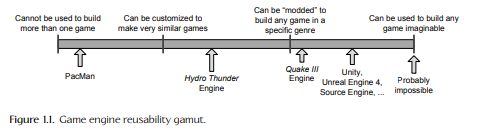
\includegraphics[width=1\linewidth]{chapters/gameEngine Usability.png}
% %     \caption{Game Engine Reusability Gamut}
% %     \label{fig:Game-Engine Reusability}
% % \end{figure}



% % Behind the curtains of any interactive application there is most likely a Game Engine. 
% % You have probably heard before about Unity and Unreal but there are many more game engines out there. Some of them are In-House, some of them are Open-Source, some of them are made for a specific Genre. But none of them is offering Built-In Machine Learning Integration. 

% % \subsection{What does a Game Engine offer?}

% % While not limited to, some of the tools we expect a game engine to offer are: 
% % \begin{enumerate}
% %     \item Input Handling
% %     \item Player Mechanics
% %     \item Game-Specific Rendering
% %     \item Collision \& Physics
% %     \item Audio Playback
% %     \item Game Cameras
% %     \item Ai \& Behaviour Management
% %     \item Online Multiplayer
% %     \item Scene Graph
% %     \item Scripting System
% %     \item Visual Effects
% % \end{enumerate}

% % \section{What is Machine Learning?}

% % \begin{enumerate}
% %     \item predicts text, predicts what the next word in a sentence would most likely be.
% %     \item it's too broad of a topic to be able to explain in detail in just one paper. And it's also not the purpose of this paper. This paper only wants to use the power of ai to simulate better npc's in games.
% %     \item for the purpose of this, i will not try to recreate or train an machine learning model, i will use an already existing one: GPT 3.5-Turbo by OpenAI.
% % \end{enumerate}

% % \subsection{Machine Learning in Game Engines}
% % \begin{enumerate}
% %     \item Inworld Origins are already working on a solution for implementing GPT4 to be used in a NPC dialogue scenario.
% %     \item There is this study where multiple GPT4 agents that can simulate believable human behavior. (Generative Agents: Interactive Simulacra of Human Behavior)
% %     % https://arxiv.org/pdf/2304.03442.pdf
% %     \item Currently, there are no game engines that have Machine Learning Systems built-in. 
% % \end{enumerate}

% % \section{Scope and Objectives of the Thesis}
% % \begin{enumerate}
% %     \item exploration, development, and evaluation of a game engine that integrates GPT-based machine learning capabilities 
% %     \item explore the architecture of a game engine while building a basic one in Python using OpenGL.
% %     \item explore what it means to add machine learning capabilities to a game engine. 
% %     \item The focus of this research is on leveraging the power of natural language processing (NLP) and GPT models to enhance various aspects of game development, including storytelling, character interactions, procedural content generation, and player experiences.
% % \end{enumerate}

